%  LaTeX support: latex@mdpi.com
%  In case you need support, please attach all files that are necessary for compiling as well as the log file, and specify the details of your LaTeX setup (which operating system and LaTeX version / tools you are using).

%=================================================================
\documentclass[entropy,article,submit,moreauthors,pdftex]{mdpi}

% If you would like to post an early version of this manuscript as a preprint, you may use preprint as the journal and change 'submit' to 'accept'. The document class line would be, e.g., \documentclass[preprints,article,accept,moreauthors,pdftex]{mdpi}. This is especially recommended for submission to arXiv, where line numbers should be removed before posting. For preprints.org, the editorial staff will make this change immediately prior to posting.

%% Some pieces required from the pandoc template
\providecommand{\tightlist}{%
  \setlength{\itemsep}{0pt}\setlength{\parskip}{4pt}}
\setlist[itemize]{leftmargin=*,labelsep=5.8mm}
\setlist[enumerate]{leftmargin=*,labelsep=4.9mm}

\usepackage{longtable}

% see https://stackoverflow.com/a/47122900

%--------------------
% Class Options:
%--------------------
%----------
% journal
%----------
% Choose between the following MDPI journals:
% acoustics, actuators, addictions, admsci, aerospace, agriculture, agriengineering, agronomy, algorithms, animals, antibiotics, antibodies, antioxidants, applsci, arts, asc, asi, atmosphere, atoms, axioms, batteries, bdcc, behavsci , beverages, bioengineering, biology, biomedicines, biomimetics, biomolecules, biosensors, brainsci , buildings, cancers, carbon , catalysts, cells, ceramics, challenges, chemengineering, chemistry, chemosensors, children, cleantechnol, climate, clockssleep, cmd, coatings, colloids, computation, computers, condensedmatter, cosmetics, cryptography, crystals, dairy, data, dentistry, designs , diagnostics, diseases, diversity, drones, econometrics, economies, education, electrochem, electronics, energies, entropy, environments, epigenomes, est, fermentation, fibers, fire, fishes, fluids, foods, forecasting, forests, fractalfract, futureinternet, futurephys, galaxies, games, gastrointestdisord, gels, genealogy, genes, geohazards, geosciences, geriatrics, hazardousmatters, healthcare, heritage, highthroughput, horticulturae, humanities, hydrology, ijerph, ijfs, ijgi, ijms, ijns, ijtpp, informatics, information, infrastructures, inorganics, insects, instruments, inventions, iot, j, jcdd, jcm, jcp, jcs, jdb, jfb, jfmk, jimaging, jintelligence, jlpea, jmmp, jmse, jnt, jof, joitmc, jpm, jrfm, jsan, land, languages, laws, life, literature, logistics, lubricants, machines, magnetochemistry, make, marinedrugs, materials, mathematics, mca, medicina, medicines, medsci, membranes, metabolites, metals, microarrays, micromachines, microorganisms, minerals, modelling, molbank, molecules, mps, mti, nanomaterials, ncrna, neuroglia, nitrogen, notspecified, nutrients, ohbm, particles, pathogens, pharmaceuticals, pharmaceutics, pharmacy, philosophies, photonics, physics, plants, plasma, polymers, polysaccharides, preprints , proceedings, processes, proteomes, psych, publications, quantumrep, quaternary, qubs, reactions, recycling, religions, remotesensing, reports, resources, risks, robotics, safety, sci, scipharm, sensors, separations, sexes, signals, sinusitis, smartcities, sna, societies, socsci, soilsystems, sports, standards, stats, surfaces, surgeries, sustainability, symmetry, systems, technologies, test, toxics, toxins, tropicalmed, universe, urbansci, vaccines, vehicles, vetsci, vibration, viruses, vision, water, wem, wevj

%---------
% article
%---------
% The default type of manuscript is "article", but can be replaced by:
% abstract, addendum, article, benchmark, book, bookreview, briefreport, casereport, changes, comment, commentary, communication, conceptpaper, conferenceproceedings, correction, conferencereport, expressionofconcern, extendedabstract, meetingreport, creative, datadescriptor, discussion, editorial, essay, erratum, hypothesis, interestingimages, letter, meetingreport, newbookreceived, obituary, opinion, projectreport, reply, retraction, review, perspective, protocol, shortnote, supfile, technicalnote, viewpoint
% supfile = supplementary materials

%----------
% submit
%----------
% The class option "submit" will be changed to "accept" by the Editorial Office when the paper is accepted. This will only make changes to the frontpage (e.g., the logo of the journal will get visible), the headings, and the copyright information. Also, line numbering will be removed. Journal info and pagination for accepted papers will also be assigned by the Editorial Office.

%------------------
% moreauthors
%------------------
% If there is only one author the class option oneauthor should be used. Otherwise use the class option moreauthors.

%---------
% pdftex
%---------
% The option pdftex is for use with pdfLaTeX. If eps figures are used, remove the option pdftex and use LaTeX and dvi2pdf.

%=================================================================
\firstpage{1}
\makeatletter
\setcounter{page}{\@firstpage}
\makeatother
\pubvolume{xx}
\issuenum{1}
\articlenumber{5}
\pubyear{2019}
\copyrightyear{2019}
%\externaleditor{Academic Editor: name}
\history{Received: date; Accepted: date; Published: date}
\updates{yes} % If there is an update available, un-comment this line

%% MDPI internal command: uncomment if new journal that already uses continuous page numbers
%\continuouspages{yes}

%------------------------------------------------------------------
% The following line should be uncommented if the LaTeX file is uploaded to arXiv.org
%\pdfoutput=1

%=================================================================
% Add packages and commands here. The following packages are loaded in our class file: fontenc, calc, indentfirst, fancyhdr, graphicx, lastpage, ifthen, lineno, float, amsmath, setspace, enumitem, mathpazo, booktabs, titlesec, etoolbox, amsthm, hyphenat, natbib, hyperref, footmisc, geometry, caption, url, mdframed, tabto, soul, multirow, microtype, tikz

%=================================================================
%% Please use the following mathematics environments: Theorem, Lemma, Corollary, Proposition, Characterization, Property, Problem, Example, ExamplesandDefinitions, Hypothesis, Remark, Definition
%% For proofs, please use the proof environment (the amsthm package is loaded by the MDPI class).

%=================================================================
% Full title of the paper (Capitalized)
\Title{Characterizing the typical information curves of diverse
languages}

% Authors, for the paper (add full first names)
\Author{Josef Klafka$^{1}$, Daniel Yurovsky$^{1*}$}

% Authors, for metadata in PDF
\AuthorNames{Josef Klafka, Daniel Yurovsky}

% Affiliations / Addresses (Add [1] after \address if there is only one affiliation.)
\address{%
$^{1}$ \quad Department of Psychology, Carnegie Mellon University, 5000
Forbes Ave, Pittsburgh, PA 15213, USA; \\
}
% Contact information of the corresponding author
\corres{Correspondence: \href{mailto:yurovsky@cmu.edu}{\nolinkurl{yurovsky@cmu.edu}}}

% Current address and/or shared authorship








% The commands \thirdnote{} till \eighthnote{} are available for further notes

% Simple summary

% Abstract (Do not insert blank lines, i.e. \\)
\abstract{Optimal coding theories of language predict that speakers
should keep the amount of information in their utterances relatively
uniform under the constraints imposed by their language. But how much do
these constraints influence information structure, and how does this
influence vary across languages? We present a novel method for
characterizing the information structure of sentences across a diverse
set of languages. While the structure of English is broadly consistent
with the shape predicted by optimal coding, languages vary broadly in
their shapes and many are not consistent with this prediction. We then
show that the characteristic information curves of languages are partly
related to a variety of typological features from phonology to word
order. These results present an important step in the direction of
exploring upper bounds for the extent to which linguistic codes can be
optimal for communication.}

% Keywords
\keyword{communication; typology; language development}

% The fields PACS, MSC, and JEL may be left empty or commented out if not applicable
%\PACS{J0101}
%\MSC{}
%\JEL{}

%%%%%%%%%%%%%%%%%%%%%%%%%%%%%%%%%%%%%%%%%%
% Only for the journal Diversity
%\LSID{\url{http://}}

%%%%%%%%%%%%%%%%%%%%%%%%%%%%%%%%%%%%%%%%%%
% Only for the journal Applied Sciences:
%\featuredapplication{Authors are encouraged to provide a concise description of the specific application or a potential application of the work. This section is not mandatory.}
%%%%%%%%%%%%%%%%%%%%%%%%%%%%%%%%%%%%%%%%%%

%%%%%%%%%%%%%%%%%%%%%%%%%%%%%%%%%%%%%%%%%%
% Only for the journal Data:
%\dataset{DOI number or link to the deposited data set in cases where the data set is published or set to be published separately. If the data set is submitted and will be published as a supplement to this paper in the journal Data, this field will be filled by the editors of the journal. In this case, please make sure to submit the data set as a supplement when entering your manuscript into our manuscript editorial system.}

%\datasetlicense{license under which the data set is made available (CC0, CC-BY, CC-BY-SA, CC-BY-NC, etc.)}

%%%%%%%%%%%%%%%%%%%%%%%%%%%%%%%%%%%%%%%%%%
% Only for the journal Toxins
%\keycontribution{The breakthroughs or highlights of the manuscript. Authors can write one or two sentences to describe the most important part of the paper.}

%\setcounter{secnumdepth}{4}
%%%%%%%%%%%%%%%%%%%%%%%%%%%%%%%%%%%%%%%%%%

% Pandoc citation processing


\begin{document}
%%%%%%%%%%%%%%%%%%%%%%%%%%%%%%%%%%%%%%%%%%

\hypertarget{introduction}{%
\section{Introduction}\label{introduction}}

One of the defining features of human language is its power to transmit
information. We use language for a variety of purposes like greeting
friends, making records, and signaling group identity. These purposes
all share a common goal: Transmitting information that changes the
mental state of our listener \citep{austin1975}. For this reason, we can
describe language as a cryptographic code, one that allows speakers to
turn their intended meaning into a message that can be transmitted to a
listener, and subsequently converted by the listener back into an
approximation of the intended meaning \citep{shannon1948}.

How should we expect this code to be structured? If language has evolved
as a code for information transmission, its structure should reflect
this process of optimization \citep{anderson1989}. The optimal code
would have to work with two competing pressures: (1) For listeners to
easily and successfully decode messages sent by the speaker, and (2) For
speakers to easily code their messages and transmit them to a listener
with minimal effort and error. A fundamental constraint on both of these
processes is the linear order of spoken language--sounds are produced
one at a time and each is unavailable perceptually once it is no longer
being produced.

Humans accommodate this linear order constraint through incremental
processing: People process speech continuously as it arrives, predicting
upcoming words and building expectations about the meaning of an
utterance in real time rather than at its conclusion
\citep{kutas2011, tanenhaus1995, pickering2013}. This solution creates
new guidance for speakers. Since prediction errors can lead to severe
processing costs and difficulty integrating new information on the part
of listeners, speakers should seek to minimize prediction errors.
However, the cost of producing more predictable utterances is using more
words. Thus, the most efficient strategy is for speakers seeking to
minimize their production costs is to produce utterances that are just
at the prediction capacity of listeners without exceeding this capacity
\citep{aylett2004, genzel2002, levy2007}. In other words, speakers
should maintain a constant transmission of information, with the optimal
rate of information transfer as close to the listener's fastest decoding
rate as possible. The hypothesis that speakers follow this optimal
strategy is known as the \emph{Uniform Information Density} hypothesis.

Using information theory, a mathematical framework for formalizing
predictability, researchers have tested and confirmed this optimal
coding prediction across several levels and contexts in language
production. For example, \citet{genzel2002} provided a clever indirect
test of Uniform Information Density across sentences in a paragraph.
They showed that the predictability of successive sentences, when
analyzed in isolation, decreases, as would be expected if readers use
prior sentences to predict the content of future sentences. Thus, based
on the increasing amount of context, they found that total
predictability remains constant. At the level of individual words,
\citet{mahowald2013} showed that speakers use shorter alternatives of
more predictable words, maximizing the amount of information in each
word while minimizing the time spent on those words.\\
Other research has suggested that efficient encoding impacts how
speakers structure units between words and sentences. The inclusion of
complementizers in relative clauses \citep{jaeger2010} and the use of
contractions \citep{frank2008} are two situations in sentence formation
in which speakers can omit or reduce words to communicate more
efficiently and maximize use of the communication channel without
exceeding the listener's capacity.

How languages evolve is shaped by efficient communication as well.
\citet{piantadosi2011} showed that more easily predictable words in a
language may tend to become shorter over time, maximizing the amount of
information transmitted over the communication channel at every second
by speakers in each language. Semantic categories of words across
languages can also evolve to be structured efficiently. Categories such
as kinship terms \citep{kemp2012} maintain a trade-off between
informativeness and complexity. Structure in langauge evolves from a
trade-off between efficient and learnable encoding on the one hand and
an expressive and descriptive lexicon on the other \citep{kirby2015}.
Languages may come to efficiently describe the particular environment in
which they are spoken over the course of evolution: features of the
world that are relevant to speakers become part of a language, while
irrelevant features are disregarded \citep{perfors2014}.

However, speakers are still bound by the syntactic rules of their
language. While complementizers are often optional, determiners are not.
Similarly, speakers may have a choice about which of several
near-synonyms they produce, but they cannot choose the canonical order
of subjects, verbs, and objects. Properties of a language, like
canonical word order, impose top-down constraints on how speakers can
structure what they say. While speakers may produce utterances as
uniform in information density as their languages will allow, these
top-down constraints may create significant and unique variation across
languages.

How significant are a language's top-down constraints on determining how
its speakers structure their speech? \citet{yu2016} analyzed how the
information in words of English sentences of a fixed length varies with
their order in the sentence (e.g.~first word, second word, etc). They
found a surprising non-linear shape, and argued that this shape may
arise from top-down grammatical constraints in the English language. In
this paper, we replicate their analysis, and then extend their ideas. We
ask: (1) Whether this shape is affected by the amount of context
leveraged in prediction, (2) Whether this shape varies across written
and spoken contexts, and (3) Whether this shape is broadly
characteristic of a diverse set of languages or varies predictably from
language to language. We find that languages are characterized by
highly-reliable but cross-linguistically variable information structures
that co-vary with top-down linguistic features. However, using
sufficient predictive context partially flattens these shapes across
languages, in accord with predictions of the Uniform Information Density
hypothesis.

\hypertarget{study-1-the-shape-of-information-in-written-english}{%
\section{Study 1: The Shape of Information in Written
English}\label{study-1-the-shape-of-information-in-written-english}}

\citet{genzel2002} performed an influential early test of the Uniform
Information Density hypothesis, analyzing the amount of information in
successive sentences in a corpus. They reasoned that if speakers keep
the amount of information in each sentence constant, but readers of the
text process each successive sentence in the context of the prior
sentences, then a predictive model that does not have access to this
prior context should find each successive sentence more surprising. To
test this hypothesis, they used a simple n-gram model in which the
surprisal of each word is computed as the probability of it following
each of the prior n-words. They found that the surprisal-per-word of
sentences later in an article was higher than sentences earlier in the
same article.

\citet{yu2016} applied this same logic to each word within sentences.
They reasoned that if speakers were processing each word in the context
of all prior words in the sentence, but their predictive model ignored
this context by considering the base-rate entropy of each word, they
would observe the same monotonically increasing surprisal as a function
of word position within each sentence. However, this is not what they
observed. Instead, they found a characteristic three-step distribution:
Words early in an utterance had very low information, then information
was constant throughout most of the utterance, then there was a slight
dip, and finally a steep rise for the final word. \citet{yu2016}
interpreted this uneven information curve as evidence against the
Uniform Information Density Hypothesis. Unlike Genzel and Charniak's
results, information plateaued in the middle of sentences and then
dipped instead of rising throughout.

However, \citet{yu2016}'s analysis leaves some open questions. First,
they used an unusual metric to quantify the information in each word.
They computed the average surprisal of all the words in a given word
position, computed only within that position, and weighted by how many
times each word occurs in that position. Their formula is given by
\(\text{H}(X) = -\sum_{w}P(w \in X) \log P(w)\), where \(X\) is a word
position (e.g.~first words, fifth words, final words) and \(w\) is a
word occuring in position \(X\). If the goal is to consider the
surprisal of each word in a model that does not use prior context, then
the model should not consider sentence position either. Second, with the
exception of the small dip that appears near the end of the sentence,
the shape is roughly consistent with the predicted monotonically
increasing per-word surprisal. Third, it is difficult to know whether
the characteristic shape generalizes across sentences of all lengths,
and not just the three particular lengths that \citet{yu2016} analyzed.
Finally, it would be ideal to estimate the characteristic information
profiles of sentences when context is considered, and not just in the
absence of the context of prior words. That is, ideally we could observe
the uniform surprisal of words directly for a model of the reader and
not just indirectly for a model of a context-less reader.

In Study 1, we attempt to resolve these issues. We first replicate Yu et
al.'s analysis using a standard unigram language model. We then use a
trigram model to show that the information in English sentences is
significantly more uniform when words are processed in context. Finally,
we introduce a method for aggregating across sentences of different
lengths to produce a single characteristic profile for sentences of
English, and show that they are broadly consistent with a Uniform
Information Density prediction akin to \citet{genzel2002}.

\hypertarget{method}{%
\subsection{Method}\label{method}}

\hypertarget{data}{%
\subsubsection{Data}\label{data}}

Following \citet{yu2016}, we selected the British National Corpus (BNC)
to estimate the information in English sentences \citep{leech1992}. The
BNC is an approximately 100 million word corpus consisting of mainly of
written (90\%) with some spoken transcriptions (10\%) of English
collected by researchers at Oxford University in the 1980s and 1990s.
The BNC is intended to be representative of British English at the end
of the 20th century, and contains a wide variety of genres
(e.g.~newspaper articles, pamphlets, fiction novels, academic papers).

We began with the XML version of the corpus, and used the
\texttt{justTheWords.xsl} script provided along with the corpus to
produce a text file with one sentence of the corpus on each line.
Compound words (like ``can't'') were combined, and all words were
converted to lowercase before analysis. This produced a corpus of just
over six million utterance of varying lengths. From these, we excluded
utterances that were too short to allow for reasonable estimation of
information shape (fewer than 5 words), and utterances that were
unusually long (more than 45 words). This exclusion left us with 89.83\%
of the utterances (Fig \ref{fig:bnc-lengths}).

\begin{figure}[tb]

{\centering 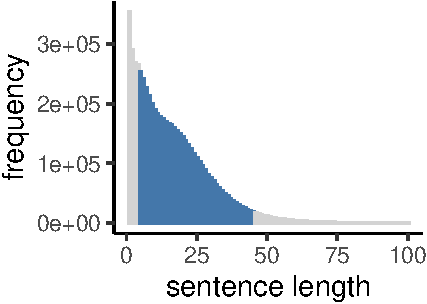
\includegraphics{figs/bnc-lengths-1} 

}

\caption{The distribution of sentence lengths in the British National Corpus (BNC). We analyzed sentences of length 5-45 (colored).}\label{fig:bnc-lengths}
\end{figure}

\hypertarget{models}{%
\subsubsection{Models}\label{models}}

To estimate how information is distributed across utterances, we
computed the lexical surprisal of words in each position of English
sentences under two different models. First, we estimated a unigram
model which considers each word independently. This unigram surprisal
measure is a direct transformation of the word's frequency and thus less
frequent words are more surprising.

\[\text{surprisal}(\text{word}) = -\log P(\text{word})\]

Second, we estimated a trigram model in which the surprisal of a given
word (\(w_i\)) encodes how unexpected it is to read it after reading the
prior two words (\(w_{i-1}\) and \(w_{i-2}\)):

\[\text{surprisal}(w_{i}) = -log P(w_i|w_{i-1},w_{i-2})\]

This metric encodes the idea that words that are low frequency in
isolation (e.g.~``meatballs'') may become much less surprising in
certain contexts (e.g.~``spaghetti and meatballs'') but more surprising
in others (e.g.~``coffee with meatballs''). Because the problem of
estimating probabilities grows combinatorically with the number of prior
words due to sparsity, we chose a trigram rather than a quadgram model
as in \citet{genzel2002}. In practice, trigram models perform well as an
approximation \citep[see e.g.][]{chen1999, smith2013}.

We estimated these models using the KenLM toolkit \citep{heafield2013}.
Each utterance was padded with a special start-of-sentence token
``\(\left<s\right>\)'' and end of sentence token
``\(\left</s\right>\)''. Trigram estimates did not cross sentence
boundaries, so for example the surprisal of the second word in an
utterances was estimated as
\(\text{surprisal}(w_{2}) = -P(w_2|w_{i},\left<s\right>)\).

Naïve trigram models will underestimate the surprisal of words in
low-frequency trigrams (e.g.~if the word ``meatballs'' appears only once
in the corpus following exactly the words ``spaghetti and'', it is
perfectly predictable from its prior two words). To avoid this
underestimation, we used modified Kneser-Ney smoothing as implemented in
the KenLM toolkit \citep{heafield2013}. Briefly, this smoothing
technique discounts all ngram frequency counts, which reduces the impact
of rare ngrams on probability calculations, and interpolates lower-order
ngrams into the calculations. These lower-order ngrams are weighted
according to the number of distinct contexts they occur as a
continuation (e.g.~``Francisco'' may be a common word in a corpus, but
likely only occurs after ``San'' as in ``San Francisco'', so it receives
a lower weighting). For a thorough explanation of modified Kneser-Ney
smoothing, see \citet{chen1999}.

In order to prevent overfitting, we computed the surprisal of words in
sentences using cross-validation. We divided the corpus into 10
sub-corpora of equal lengths. For each sub-corpus, we fit the unigram
and trigram models on all other subcorpora, and then used this model to
estimate the surprisal of words in this corpus.

\hypertarget{characteristic-information-curves}{%
\subsubsection{Characteristic information
curves}\label{characteristic-information-curves}}

To develop a characteristic information curve for sentences in the
corpus, we needed to aggregate sentences that varied dramatically in
length (Figure \ref{fig:bnc-plots}A). We used Dynamic Time Warping
Barycenter Averaging (DBA), an algorithm for finding the average of
sequences that share and underlying pattern but vary in length
\citep{petitjean2011}.

Dynamic Time Warping is a method for calculating an alignment between
two sequences in which one can be produced by warping the other.
Canonically, there is a template sequence (e.g.~a known vowel's acoustic
profile, a known walker's motion-capture limb positions) and a set of
unknown sequences that may be new instances of the template sequence
produced by perturbations in speed or acceleration (e.g.~extending pr
shortening the vowel, walking faster or slower). Dynamic time warping
works by finding a partial match between the known template and unknown
instance under the constraint that each point in the instance must come
from a point in the template, and that the ordering of points must be
preserved, but that multiple points in the sequence can match one point
in the template (i.e.~lengthening) and multiple points in the template
can match one point in the sequence (i.e.~shortening).

Dynamic time warping barycenter averaging inverts standard dynamic time
warping, discovering a latent invariant template from a set of sequences
rather than identifying new instances of a known template. We used DBA
to discover the short sequence of surprisal values that characterized
the surprisal curves common to sentences of varying sentence lengths. We
first averaged individual sentences of the same length together and then
applied the DBA algorithm to this set of average sequences.

We use the implementation of DBA in the Python package tslearn
\citep{tavenard2017}, which fits the barycenter to a time-series dataset
through the expectation-maximization algorithm \citep[EM][]{moon1996}.
DBA in this implementation allows us to specify the size of the
barycenter. Because of the characteristic shape observed by
\citet{yu2016} and that we also found in our data (Fig
\ref{fig:bnc-lengths}), we chose a barycenter of length 5 to capture the
varying information slopes across sentences. However, all of the results
we report in this Study and in others were similar for barycenters of
varying lengths.

\hypertarget{results-and-discussion}{%
\subsection{Results and Discussion}\label{results-and-discussion}}

\begin{figure}[tb]

{\centering 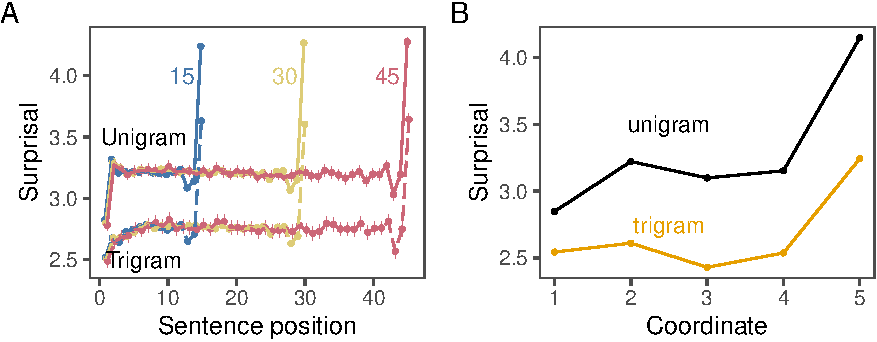
\includegraphics{figs/bnc-plots-1} 

}

\caption{(A) Surprisal by sentence position of length 15, 30, and 45 sentences in the British National Corpus under unigram and trigram surprisal models. Error bars indicate 95\% confidence intervals (tiny due to sample size). (B) Characteristic information curves produced by the DBA algorithm averaging over all sentence lengths in each corpus.}\label{fig:bnc-plots}
\end{figure}

We began by replicating Yu et al.'s analyses with a standard unigram
model, examining the surprisal of words in sentence of length 15, 30,
and 45 as they did. In line with their findings, we found a reliably
non-linear shape in sentences of all 3 lengths, with the information in
each word rising for the first two words, plateauing in the middle of
sentences, dipping in pen-ultimate position, and rising steeply on the
final word (Figure \ref{fig:bnc-plots}A). Qualitatively, we found the
same shape in utterances of all other lengths we sampled, from
utterances with 5 words to utterances with 45 words.

In comparison, under the trigram model we observed 3 major changes.
First, each word contained significantly less information. This is to be
expected as the knowing two prior words makes it much easier to predict
the next word. Second, the fall and peak at the ends of utterances was
still observable, but much less pronounced. Finally, the first word of
each sentence was now much more surprising than the rest of the words in
the sentence, because the model had only the start of sentence token
\(\left<s\right>\) to use as context. Thus, the trigram model likely
overestimates the information for humans reading the first word.
Together, these results suggest that \citet{yu2016} overestimated the
non-uniformity of information in sentences. Nonetheless, the final words
of utterances do consistently contain more information than the other
words.

Figure \ref{fig:bnc-plots}B shows the barycenters produced by the
dynamic time warping barycenter averaging algorithm (DBA). The algorithm
correctly recovers both the initial and final rise in information under
the unigram model, and the initial fall and smaller final rise in the
trigram model. We take this as evidence that (1) these shapes are
characteristic of all lengths, and (2) that DBA effectively recovers
characteristic information structure.

In sum, the results of Study 1 suggest that sentences of written English
have a characteristic non-uniform information structure, with
information rising at the ends of sentences. This structure is more
pronounced when each word is considered in isolation, but some of the
structure remains even when each word is considered in context. These
results are broadly consistent with the predictions of a Uniform
Information Density Account: Information increases over the course of
sentences, but approaches uniformity as more context is considered.

Is this structure unique to written English, or does it characterize
spoken English as well? In Study 2, we apply this same analysis to two
corpora of spoken English--the first of adults speaking to other adults,
and the second of adults and children speaking to each other.

\hypertarget{study-2-information-in-spoken-english}{%
\section{Study 2: Information in Spoken
English}\label{study-2-information-in-spoken-english}}

Spoken language is different from written language in several respects.
First, the speed at which it can be processed is constrained by the
speed at which it is produced. Second, speech occurs in a multimodal
environment, providing listeners information from a variety of sources
beyond the words conveyed (e.g.~prosody, gesture, world context).
Finally, both words and sentence structures tend to be simpler in spoken
language than written language as they must be produced and processed in
real time \citep{christiansen2016}. Thus, sentences of spoken English
may have different information curves than sentences of written English.

The language young children hear is further different from the language
adults speak to each other. Child-directed speech tends to simpler than
adult-directed speech on a number of dimensions including the lengths
and prosodic contours of utterances, the diversity of words, and the
complexity of syntactic structures \citep{snow1972}. The speech produced
by young children is even more distinct from adult-adult speech, replete
with simplifications and modifications imposed by their developing
knowledge of both the lexicon and grammar \citep{clark2009}. In Study 2,
we ask whether spoken English--produced both by adults and children--
has the same characteristic information shape as written English.

\hypertarget{method-1}{%
\subsection{Method}\label{method-1}}

\hypertarget{data-1}{%
\subsubsection{Data}\label{data-1}}

To estimate the information in utterances of adult-adult spoken English,
we used the Santa Barbara Corpus of Spoken American English, a \(\sim\)
250,000 word corpus of recordings of naturally occurring spoken
interactions from diverse regions of the United States
\citep{du-bois2000}. For parent-child interactions, we used all of the
North American English corpora in the Child Language Data Exchange
System (CHILDES) hosted through the childes-db interface
\citep{macwhinney2000, sanchez2019}. We selected for analysis all
\(\sim\) 1 million utterances produced by children (mostly under the age
of five), and \(\sim\) 1.7 million utterances produced by the parents of
these children.

\hypertarget{models-1}{%
\subsubsection{Models}\label{models-1}}

All pre-processing and modeling details were identical to Study 1 except
for the selection of sentences for analysis. Because the utterances in
both the Santa Barbara Corpus and CHILDES were significantly shorter
than the sentences in the British National Corpus, we analyzed all
utterances of at least 5 and most 15 words (see Fig.
\ref{fig:spoken-figs}A). Models were estimated separately for each of
the 3 corpora.

\hypertarget{results-and-discussion-1}{%
\subsection{Results and Discussion}\label{results-and-discussion-1}}

\begin{figure}[tb]

{\centering 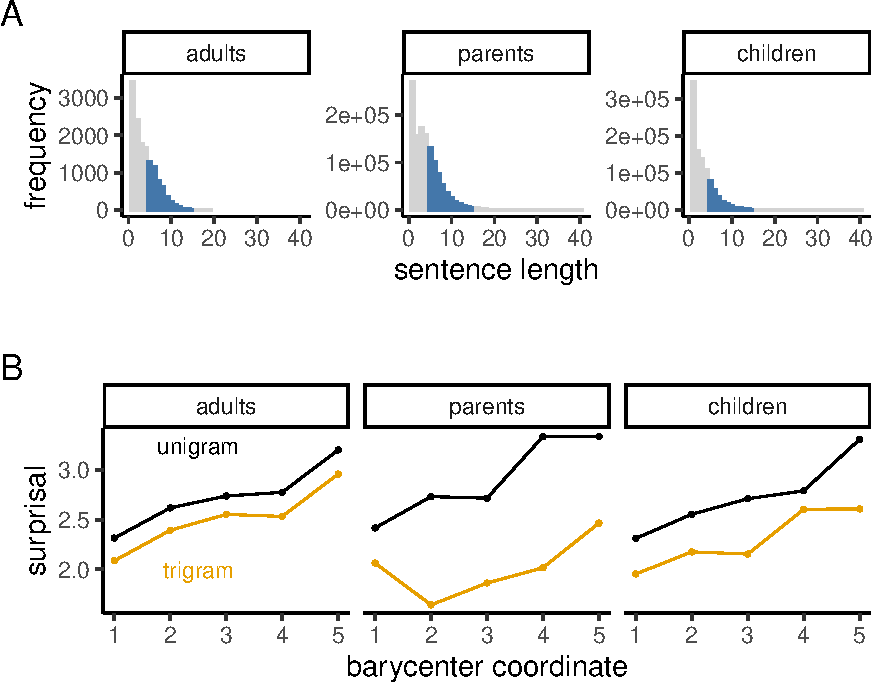
\includegraphics{figs/spoken-figs-1} 

}

\caption{(A) The distribution of sentence lengths in the spoken English corpora: Adults in Santa Barbara, and parents and children in CHILDES. We analyzed sentences of length 5-15 (colored). (B) Charateristic surprisal curves for these corpora.}\label{fig:spoken-figs}
\end{figure}

The information curves found in adults-adult utterances were quite
similar to those of parent-child utterances and child-parent utterances
(Fig. \ref{fig:spoken-figs}B). Under the unigram model, information rose
steeply in the beginnings of utterances, was relatively flatter in the
middle of utterances, and the rose even more steeply at the ends. Under
the trigram model, the curve was nearly identical. Both curves were
similar in shape to the characeristic curve for written English
estimated in Study 1.

Curves for parent and child speech were similar to those of adults with
some small differences. Unigram curves for both were monotonically
increasing, although the largest jump in the parent curve occurred in
the 4th barycenter position rather than the third. Trigram curves were
also broadly similar, although the parent curve dipped between first and
second position. This decreasing slope is inconsistent with the UID
prediction of monotonic increase. It is possible that this decrease is a
real feature of speech to children--parents may begin utterances to
children more variably than when they speak to other adults.

Overall, the preponderance of evidence suggests that the characteristic
shape of the information curve for spoken English is similar to that of
written English. And this appears to be approximately true in speech to
children and by children. All of these curves are broadly consistent
with predictions from a Uniform Information Density account that
information measured without context should increase, and that including
some context will reduce the rate of increase.

In Study 3 we apply this technique to a diverse set of written languages
of different families to ask whether these structures vary
cross-linguistically.

\hypertarget{study-3-language-structures-and-large-scale-data-analysis}{%
\section{Study 3: Language structures and large-scale data
analysis}\label{study-3-language-structures-and-large-scale-data-analysis}}

In Study 3, we applied the same method as in Studies 1 and 2 to a
diverse set of over two hundred natural languages represented on
Wikipedia. In our prior studies, we found that the distribution of
information in sentences of English is broadly consistent with
predictions of a Uniform Information Density account: Information
roughly rises over sequential words in a sentence, and further
information rises more slowly when more prior context is used to predict
the next word. In Study 3 we ask whether this same pattern characterizes
natural languages in general, and whether variability in the
characteristic information curves of languages is related to their
typological features.

\hypertarget{method-2}{%
\subsection{Method}\label{method-2}}

\hypertarget{data-2}{%
\subsubsection{Data}\label{data-2}}

To measure cross-linguistic variation in the structure of information
across sentences, we constructed a corpus of Wikipedia articles using
the Wikiextractor tool from the Natural Language Text Analytics (TANL)
pipeline \citep{attardi2010}. We retained all languages with at least
10,000 articles, resulting in data from a set of 234 languages from 29
families.

To understand how potential variation in information curve shape are
related to the structure of these languages, we used the typological
feature information for these languages available in the World Atlas of
Language Structures \citep[WALS,][]{wals}. The WALS database has data
for \(144\) typological features in thousands of languages from across
the world. These features describe aspects of morphology, syntax,
phonology, etymology and semantics--in short the features describe the
structures in each language.

There are several categories of WALS features. Phonology features
describe sounds, stress, intonation, and syllable structure in each
language. Nominal categories describe the morphology and semantics of
nouns, including features for cases, definiteness and plurals. Verbal
categories describe analogous verb features, focusing on tense, mood and
aspect. Nominal syntax features describe a heterogeneous collection of
noun phenomena, focusing on possessives and adjectives. Word order
features describe word order in a language, not only canonical ordering
of the subject, object and verb but also orderings of heads and
modifiers, relative clauses and other orderings. Simple clause features
describe the syntax and organization of single clauses, such as passive
and negative constructions in the language.

\hypertarget{models-2}{%
\subsubsection{Models}\label{models-2}}

Language models were estimated separately for each language using the
same procedures as in Study 1. To accommodate the variety of lengths
across language corpora, we analyzed sentences of lengths 5 to 45. Word
boundaries were assumed to be identified by spaces as in Studies 1 and
2. Wikipedia entries for all languages were hand-checked to ensure that
this assumption was appropriate to the best of our abilities, but it is
a potential source of noise in the analyses.

For each pair of languages, we derived two pairwise similarity measures.
To estimate the information structure similarity, we first centered each
language's 5-point barycenter curve (since surprisal is highly correlate
with corpus size), and then computed the cosine similarity between the
two centered curves. To compare typological similarity, we computed the
proportion of features in the World Atlas of Linguistic Structure (WALS)
on which the two languages shared the same feature value. Because WALS
is a compiled collection from the fieldwork of many linguists, rather
than a complete analysis by a single group, features vary in the number
of values they take. Some features--like Vowel Quality Inventories (2A),
have multiple features but also a natural ordering (small inventory,
medium inventory, large inventory). However, others, like others like
Position of Tense-Aspect Affixes (69A) have multiple values with no
obvious ordering (prefixes, suffixes, tone, combination with no primary,
none). For this reason, we used exact match as our distance function,
but other more sensitive metrics could be used in the future by other
researchers.

Finally, because of the collaboratie constructin of WALS, many features
are missing in many languages. For this reason, only features present in
WALS for both languages in a pair were considered for estimating their
proportion of shared features. We also attempted to address this
sparsity problem by imputing missing feature data where possible using
Multiple Imputation with Multiple correspondence Analysis
\citep[MIMCA,][]{audigier2017}. MIMCA begins with mean imputation,
converts the categorical WALS features into a numerical contingency
table with dummy coding, then repeatedly performs principle components
analysis and reconstructs the contingency table. Results of analyses
using imputed features were qualitatively to those performed on raw
features but with weaker correlations as described below. Nonetheless,
we report both measures as they may be of use in future research.

\hypertarget{results-and-discussion-2}{%
\subsection{Results and Discussion}\label{results-and-discussion-2}}

In Studies 1 and 2, we observed that characteristic information curve of
English to be generally increasing in both unigram and trigram models.
In Study 3, we first replicated this analysis on the larger English
language sample in the Wikipedia corpus (Figure \ref{fig:wiki-english}).
The unigram information curve for English estimated on Wikipedia was
nearly identical to the curve observed in the British National Corpus un
Study 1 (see Figure \ref{fig:bnc-plots}b). The trigram curve had a more
pronounced dip in the 4th coordinate, but otherwise maintained the
general shape and characteristic final rise we had previously observed.

\begin{figure}[tb]

{\centering 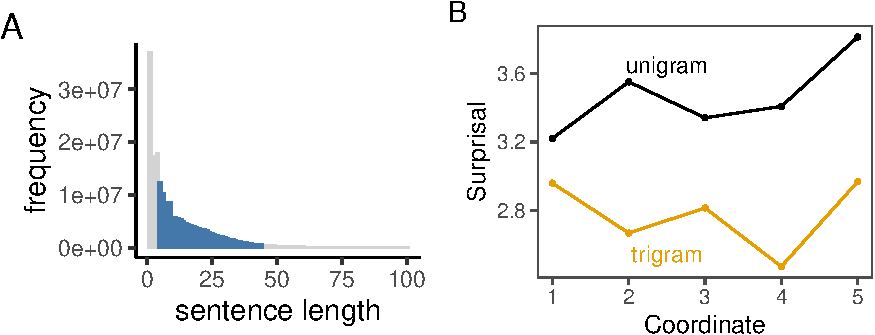
\includegraphics{figs/wiki-english-1} 

}

\caption{(A) The distribution of sentence lengths in the English Wikipedia Corpus. We analyzed sentences of length 5-45 (colored). (B) Charateristic information curves for English in the Wikipedia corpus.}\label{fig:wiki-english}
\end{figure}

This shape did not, however, characterize all of the 234 represented in
Wikpedia. Languages varied widely in the shapes of their information
curves, both in the unigram and in the trigram model. Under the unigram
model, some languages--like Spanish and German were generally increasing
like English. Others, like Hindi and Chinese, had negative slopes in
their characteristic curves, and yet others like Urdu had a mix of
positive and negative slopes. Under the trigram model, languages also
varied, with reliable negative slopes in a number of languages including
Russian and Urdu.

In lieu of presenting characteristic curves for all languages, Figure
\ref{fig:family-curves} shows the characteristic information curves for
each of the six language families in which at least 10 languages were
represented in Wikipedia. These curves were produced by first centering
the surprisal for each language so that the surprisal of the mean word
was 0 in order to deconfound differences due to corpus size, and then
applying the barycenter averaging algorithm to the curves from all
languages in the relevant family.

\begin{figure}[tb]

{\centering 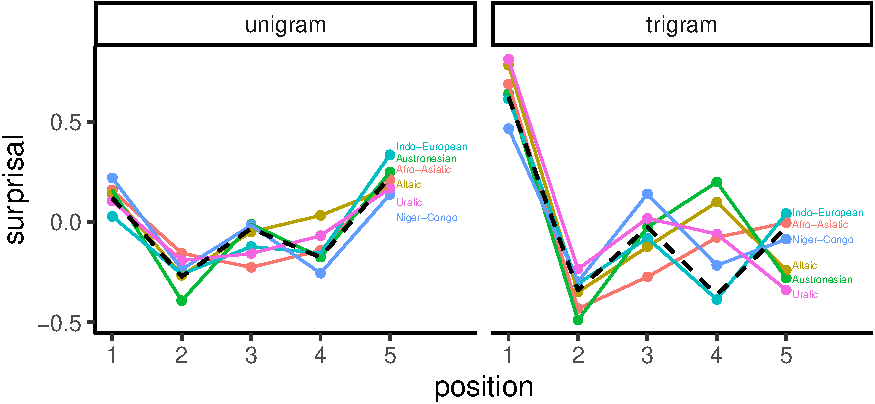
\includegraphics{figs/family-curves-1} 

}

\caption{Centered characteristic information curves for the six most frequent language families represented on Wikipedia. The dashed line shows the mean curve across all language families.}\label{fig:family-curves}
\end{figure}

Two main trends are apparent. First, no language families have curves
that are monotonically increasing, and neither does the mean curve over
all languages for either the unigram nor the trigram model. Thus, the
Uniform Information Density prediction does not appear to hold for
languages other than English. Second, information curves for distinct
families were more different from each-other under the trigram model
than the unigram model. To confirm this statistically, we computed the
variance in surprisals at each of the 5 barycenter positions across all
234 languages. The average variance across the 5 positions under the
unigram model was 0.077 with a 95\% confidence interval of {[}0.05,
0.104{]}. The average variance under the trigram model was 0.163
{[}0.113, 0.218{]}. Matching our observation, these confidence intervals
do not overlap.

\begin{figure}[tb]

{\centering 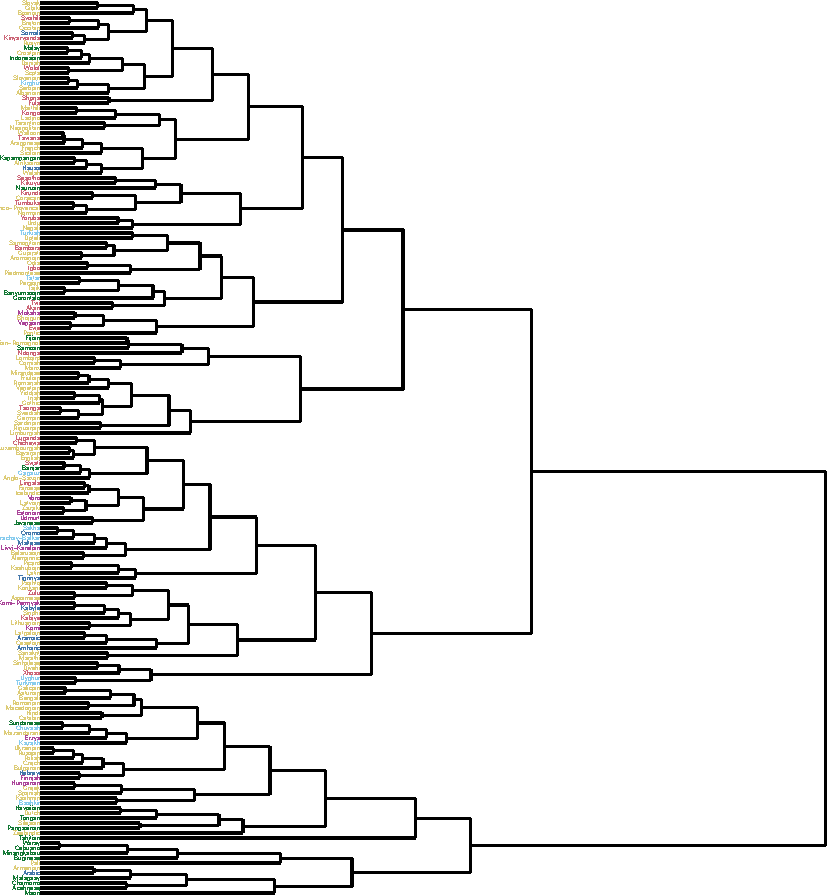
\includegraphics{figs/dendro-1} 

}

\caption{A dendrogram constructed by hierarchically clustering languages in the six most-well represented families on Wikipedia according to the similarities of their characteristic information curves. Languages are colored according to their language family.}\label{fig:dendro}
\end{figure}

Together, these results suggest that the characteristic information
curves of different languages may diverge from the UID prediction
because of the influence of idiosyncratic syntactic properties of these
languages that prevent them from being optimal codes. If this is the
case, then languages that are more similar to either phylogentically may
also have more similar information curves. Figure \ref{fig:dendro} shows
a dendrogram produced by hierarchichally clustering on the basis of
cosine similarity of information curves. All of the languages that
belong from the families shown in Figure \ref{fig:family-curves} are
represented. Although not all members of each language family are
clustered closely together, but some structure is certainly apparent.
For instance, all of the Austronesian languages are quite similar.

To test the hypothesis that linguistic similarity leads to information
curve similarity, we considered the relationship between the typological
features of languages and their characteristic information curves. For
each pair of languages, we computed the characteristic curve similarity
using cosine distance, and their typological similarity using number of
shared WALS features (both raw and imputed). Under the unigram model,
the two similarity measures were significantly but very weakly
correlated (\(r_{raw} =\) 0.056, \(t_{raw} =\) 3.786, \(p_{raw}\)
\textless{} .001; \(r_{imputed} =\) 0.025, \(t_{imputed} =\) 2.715,
\(p_{imputed} =\) .007). Under the trigram model, this correlation was
still low, but an order of magnitude stronger (\(r_{raw} =\) 0.203,
\(t_{raw} =\) 13.899, \(p_{raw}\) \textless{} .001; \(r_{imputed} =\)
0.124, \(t_{imputed} =\) 13.349, \(p_{imputed}\) \textless{} .001).

To understand which typological features contribute to these
similarities, we split the WALS features by type, with categories such
as nominative categories and nominative syntax describing morphology
while word order describes subject-verb-object and head-modifier word
orders. Figure \ref{fig:type-cors} shows the correlation between the
similarity of information curves under both the unigram and trigram
models and the number of features of each of these types two-languages
shared. Under the unigram model, word order features and possibly
nominal category features appear to predict information curve
similarity. In contrast, under the trigram model, all features types
except for possibly nominal syntax are reliably correlated with
information curve similarity. Thus, almost all of the typological
features represented in WALS are reflected in the characteristic
information curves of languages. These analyses suggest that languages
may be pressured to be optimal codes, but that the historical influences
on the structures of languages may put in place limits on the degree of
efficiency of these codes.

\begin{figure}[tb]

{\centering 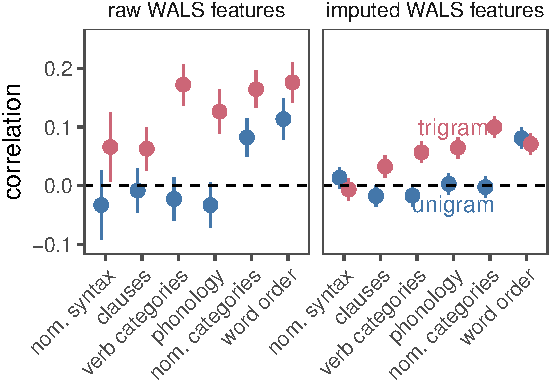
\includegraphics{figs/type-cors-1} 

}

\caption{Pairwise correlations between languages' normalized information curves and the number of linguistic features they share of each type. Error bars indicate 95\% confidence intervals.}\label{fig:type-cors}
\end{figure}

\hypertarget{general-discussion}{%
\section{General Discussion}\label{general-discussion}}

Why do languages have the regularities we observe in them? The
particular features of any one language may owe their origin to a
diverse set of ecological pressures, features of the population of
speakers, or other idiosyncratic causes
\citep{maddieson2015, lupyan2010}. Despite the difficulty of explaining
variability across languages, significant progress in explaining
universals has been made by taking an optimal coding perspective on
language. If languages have evolved to be efficient codes for
transmitting information, they should all have certain predictable
features \citep{anderson1989, shannon1948}.

One such predicted feature has been called the Uniform Information
Density hypothesis--speakers should try to keep the amount of
information they transmit constant rather than produce spikes that lead
to difficulties in comprehension
\citep{aylett2004, genzel2002, levy2007}. \citet{genzel2002} developed a
clever method to confirm this prediction at the level of sentences in an
article, and a variety of other results have confirmed similar results
at a variety of other levels of language
\citep[e.g.][]{jaeger2010, van-son2005}. However, recent work from
\citet{yu2016} suggests that this prediction may not hold at the level
on subsequent words within a sentence.

In this paper, we build the method employed by \citet{yu2016} to develop
a novel method for quantifying how information is typically distributed
across the words of a sentence. We showed that English--whether written
or spoken, whether produced by adults or children--has a prototypical
information structure. Further, this prototypical structure is broadly
in line with the predictions of the Uniform Information Density
Hypothesis.

However, the same prediction does not hold for many other languages.
Instead, the characteristic information curves of languages are at least
partially influenced by a variety of features of their typological
structure (e.g.~word order). These top-down constraints appear to place
limits on the extent to which languages can approximate optimal codes.
These results represent a small first step towards answering the
question of how much these constraints shape speakers' productions, and
how speakers interact with them.

% %%%%%%%%%%%%%%%%%%%%%%%%%%%%%%%%%%%%%%%%%%
% %% optional
% \supplementary{The following are available online at www.mdpi.com/link, Figure S1: title, Table S1: title, Video S1: title.}
%
% % Only for the journal Methods and Protocols:
% % If you wish to submit a video article, please do so with any other supplementary material.
% % \supplementary{The following are available at www.mdpi.com/link: Figure S1: title, Table S1: title, Video S1: title. A supporting video article is available at doi: link.}

\vspace{6pt}

%%%%%%%%%%%%%%%%%%%%%%%%%%%%%%%%%%%%%%%%%%
\acknowledgments{This research was funded by a James S McDonnell
Foundation Scholar Award to DY.}

%%%%%%%%%%%%%%%%%%%%%%%%%%%%%%%%%%%%%%%%%%
\authorcontributions{J.K. and D.Y. conceive and designed the
experiments; J.K. and D.Y. performed the experiments; J.K. and D.Y.
analyzed the data; J.K. and D. Y. wrote the paper.}

%%%%%%%%%%%%%%%%%%%%%%%%%%%%%%%%%%%%%%%%%%
\conflictsofinterest{The authors declare no conflict of interest.}

%%%%%%%%%%%%%%%%%%%%%%%%%%%%%%%%%%%%%%%%%%
%% optional
\abbreviations{The following abbreviations are used in this manuscript:\\

\noindent
\begin{tabular}{@{}ll}
BNC & British National Corpus \\
SBC & Santa Barbara Corpus of Spoken American English \\
DBA & Dynamic Time Warping Barycenter Averaging \\
CHILDES & Child Language Data Exchange System \\
WALS & World Atlas of Linguistic Structure \\
MIMCA & Multiple Imputation Multiple Correspondence Analysis \\
\end{tabular}}


%%%%%%%%%%%%%%%%%%%%%%%%%%%%%%%%%%%%%%%%%%
% Citations and References in Supplementary files are permitted provided that they also appear in the reference list here.

%=====================================
% References, variant A: internal bibliography
%=====================================
%\reftitle{References}
%\begin{thebibliography}{999}
% Reference 1
%\bibitem[Author1(year)]{ref-journal}
%Author1, T. The title of the cited article. {\em Journal Abbreviation} {\bf 2008}, {\em 10}, 142--149.
% Reference 2
%\bibitem[Author2(year)]{ref-book}
%Author2, L. The title of the cited contribution. In {\em The Book Title}; Editor1, F., Editor2, A., Eds.; Publishing House: City, Country, 2007; pp. 32--58.
%\end{thebibliography}

% The following MDPI journals use author-date citation: Arts, Econometrics, Economies, Genealogy, Humanities, IJFS, JRFM, Laws, Religions, Risks, Social Sciences. For those journals, please follow the formatting guidelines on http://www.mdpi.com/authors/references
% To cite two works by the same author: \citeauthor{ref-journal-1a} (\citeyear{ref-journal-1a}, \citeyear{ref-journal-1b}). This produces: Whittaker (1967, 1975)
% To cite two works by the same author with specific pages: \citeauthor{ref-journal-3a} (\citeyear{ref-journal-3a}, p. 328; \citeyear{ref-journal-3b}, p.475). This produces: Wong (1999, p. 328; 2000, p. 475)

%=====================================
% References, variant B: external bibliography
%=====================================
\reftitle{References}
\externalbibliography{yes}
\bibliography{mybibfile.bib}

%%%%%%%%%%%%%%%%%%%%%%%%%%%%%%%%%%%%%%%%%%
%% optional

%% for journal Sci
%\reviewreports{\\
%Reviewer 1 comments and authors’ response\\
%Reviewer 2 comments and authors’ response\\
%Reviewer 3 comments and authors’ response
%}

%%%%%%%%%%%%%%%%%%%%%%%%%%%%%%%%%%%%%%%%%%
\end{document}
